\documentclass{beamer}
\usepackage[utf8]{inputenc}

\usetheme{Madrid}
\usecolortheme{default}

% For the bibliography
\usepackage{bibentry}
\renewcommand{\refname}{Literature}
\usepackage[style=nature, backend=biber]{biblatex}
\preto\fullcite{\AtNextCite{\defcounter{maxnames}{99}}}
\addbibresource{references.bib}

% For Polish langage
\usepackage[T1]{fontenc}
% \usepackage[polish]{babel}

% For strikethrough text
\usepackage{ulem}

% For tables
\usepackage{multirow}
\usepackage{pdflscape}
\usepackage{colortbl}
\usepackage{tabulary}
\usepackage{etoolbox}
\usepackage{makecell}
\newcolumntype{P}[1]{>{\centering\arraybackslash}p{#1}}

% For figures
\usepackage{caption}
\usepackage{subcaption}

% For math
\usepackage{amsmath,amsfonts}

% Title page
\title[WAW 2024]{19th Workshop on Modelling and Mining Networks}
\subtitle{
    Network Diffusion --- Framework to Simulate Spreading Processes in Complex
    Networks
}
\author[Micha{\l} Czuba et al.]{
    Micha{\l} Czuba \inst{1},
    Mateusz Nurek \inst{1},
    Damian Serwata \inst{1},
    Yu-Xuan Qi \inst{2},
    Mingshan Jia \inst{2},
    Katarzyna Musial \inst{2},
    Rados{\l}aw Michalski \inst{1},
    Piotr Br{\'o}dka \inst{1}
}
\institute[]{
  \inst{1} Wroc{\l}aw University of Science and Technology\\
  \inst{2} University of Technology Sydney
}
\date[21.05.2024]{21.05.2024}
\logo{
\includegraphics[height=0.5cm]{figures/nsl.pdf}}



% What will be displayed at the beginning of each section and at the end of document
% \AtBeginSection[]
% {
%   \begin{frame}
%     \begin{center}
%         \huge \secname
%     \end{center}
%   \end{frame}
% }
\AtEndDocument{
    \addtocounter{framenumber}{-1}
    \begin{frame}[c]
        \begin{center}
            \huge Thank you for your attention!
        \end{center}
        \begin{figure}
            \centering
            
\includegraphics[width=5cm]{figures/qr_code.png}
        \end{figure}
    \end{frame}
}

\begin{document}

\frame{\titlepage}

\begin{frame}
    \frametitle{Agenda}
    \tableofcontents
\end{frame}

\section{What is this talk about?}
% - we woud like to present a package 
% - for whom
% - why
% - 

\section{Example I}

\section{Example II}

\section{Resources and references}

\begin{frame}[fragile]{\secname}
    The library can be installed via:
    \begin{center}
        \large
        \begin{verbatim}
            pip install network-diffusion
        \end{verbatim}
    \end{center}
    Other useful resources have also been published:
    \begin{itemize}
        \item PyPI website: \url{pypi.org/project/network-diffusion}
        \item GitHub page: \url{github.com/anty-filidor/network_diffusion}
        \item Reference guide: \url{network-diffusion.readthedocs.io}
        \item A preprint of the paper: \url{arxiv.org/abs/2405.18085}
    \end{itemize}
\end{frame}


% - Slajd tytułowy
% - Po co network diffusion
% - Przykład I - ltm
% - Przykład II - sir+ua
% - Slajd z linkami do dokumentacji / pypi / githuba
% - Koniec



% \begin{frame}{\secname}
%     Influence maximisation problem can be considered in various contexts:
%     dynamics of political opinions, marketing campaigns, spread of epidemics,
%     computer viruses, etc.
%     \begin{figure}
%         \centering
%         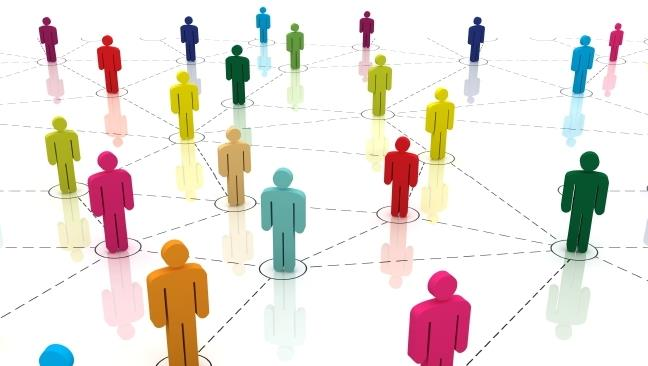
\includegraphics[width=.7\textwidth]{figures/social_network.jpg}
%         \caption{Artistic representation of a social network.\footnote{Source: \url{
%         www.uniroma3.it/articoli/seminario-biased-opinion-dynamics-when-the-devil-is-in-the-details-138122}
%         }}
%     \end{figure}
% \end{frame}

% \subsection{Research Environment \& COVID-19 Precaution Analysis}

% \begin{frame}{\subsecname}
%     \fullcite{czuba2024networkdiffusion}
%     \begin{itemize}
%         \item paper published in the journal "Big Data Mining and Analysis", 
%             20 points MNiSW, Impact Factor 13,
%         \item this is an extension and continuation of the work presented in the 
%         article "Simulating Spreading of Multiple Interacting Processes in Complex
%         Networks" (DSAA 2022),
%         \item article accepted for presentation at:
%         \begin{itemize}
%             \item WAW 2024 (Warsaw, Poland) --- oral presentation,
%             \item NetSci 2024 (Quebec, Canada) --- poster,
%             \item IC2S2 2024 (Philadelphia, USA) --- oral presentation.
%         \end{itemize}
%     \end{itemize}
% \end{frame}

% \begin{frame}{\subsecname}
%     Motivation:
%     \begin{itemize}
%         \item we have presented a significantly extended research environment,
%         \textit{Network Diffusion}, along with a detailed description of new 
%         functionalities,
%         \item we wanted to conduct the preliminary study for network controllability
%         methods used in the problem of influence maximisation in multilayer networks,
%         \item we wanted to show the usecases of the environment on the real problems,
%         \item the environment serves as a "boilerplate" for currently ongoing
%         research (network controllability / generalisation of ML-methods in 
%         influence maximisation).
%     \end{itemize}
% \end{frame}

% \begin{frame}{\subsecname}
%     Contribution -- we have presented the "Network Diffusion" framework that 
%     allows for:
%     \begin{columns}[T]
%         \begin{column}{.5\textwidth}
%             \begin{itemize}
%                 \item analysis of multilayer and temporal networks,
%                 \item simulation of spreading processes,
%                 \item use of ready-made methods for selecting initial nodes/actors
%                 in Inf. Max.,
%                 \item easy implementation of custom spreading processes,
%                 \item compatibility with the most popular Python library for 
%                 network analysis - NetworkX.
%             \end{itemize}
%         \end{column}
%         \begin{column}{.5\textwidth}
%             \vspace{1em}
%             \centering
%             \includegraphics[width=\textwidth]{figures/pypi.png}
%         \end{column}
%       \end{columns}
% \end{frame}

% \begin{frame}{\subsecname}
%     Contribution -- we conducted a study on the disease-awareness model (SIR-UA)
%     to assess the effectiveness of measures against the spread of COVID-19:
%     \textcolor{red}{lockdown}, \textcolor{red}{wearing masks}, or \textcolor{red}{no restrictions}
%     based on real parameters published in medical scientific literature (e.g., Lancet):
%     \begin{columns}[T]
%         \captionsetup{font=scriptsize}
%         \begin{column}{.5\textwidth}
%             \begin{table}
%             \centering
%             \caption{Transition weights with explanation.}
%             \resizebox{1\textwidth}{!}{%
%             \begin{tabular}{c|c|p{4cm}}
%             Symbol & Formula / Value & Description \\ \hline
%             $\alpha$ & $0.19$ & probability of infection for unaware agents \\ \hline
%             $\alpha'$ & \makecell{
%                 $\lambda\alpha;$ \\ \textcolor{red}{$\pmb{\lambda \in \{ 0.1, 0.35, 1\}}$}
%             } & probability of infection for aware agents \\ \hline
%             $\beta$ & $0.10$ & probability of recovery \\ \hline
%             $\gamma$ & $0.01$ & probability of awareness for uninfected agents \\ \hline
%             $\delta$& $\gamma + 1 - 0.3$ & probability of awareness for infected agents \\ \hline
%             \end{tabular}%
%             }
%             \end{table}
%         \end{column}
%         \begin{column}{0.5\textwidth}
%         \begin{figure}
%             \centering
%             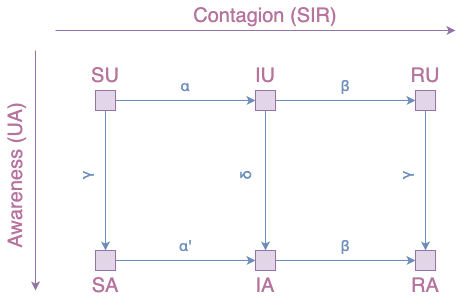
\includegraphics[width=\textwidth]{figures/sir_ua/sir_ua.png}
%             \caption{State and transition graph for SIR-UA.}
%         \end{figure}
%         \end{column}
%       \end{columns}
% \end{frame}

% \begin{frame}{\subsecname}
%     Conclusions -- for each of the investigated networks (ER, SF, real), 
%     sanitary restrictions have an impact on the peak number of infections, which
%     is of significant importance in the context of healthcare system capacity
%     during epidemics.
%     \begin{figure}[ht]
%         \centering
%         % \includegraphics[width=.8\textwidth]{figures/sir_ua/sir_ua_aucs.png}
%         % \includegraphics[width=.8\textwidth]{figures/sir_ua/sir_ua_sf.png}
%         \includegraphics[width=.8\textwidth]{figures/sir_ua/sir_ua_er.png}
%         \caption{Infection (L) and awareness (R) curves for ER network.}
%     \end{figure}
% \end{frame}


% \subsubsection{Influence Maximisation Problem}

% \begin{frame}{\subsubsecname}
%     \begin{figure}
%         \centering
%         \includegraphics[width=.7\textwidth]{figures/im_framework.pdf}
%         \caption{Components needed to define the influence maximisation problem.}
%     \end{figure}
% \end{frame}

% \begin{frame}{\subsubsecname}
%     We can distinguish three groups of methods for selecting seed set (i.e. 
%     ininitally active agenst "patients zero"):
%     \begin{itemize}
%         \item simulation-based
%         \begin{itemize}
%             \item ...
%         \end{itemize}
%         \item heuristic-based
%         \begin{itemize}
%             \item \textbf{rank refinement}
%             \item model reduction
%         \end{itemize}
%         \item mixed approaches
%         \begin{itemize}
%             \item ...
%         \end{itemize}
%     \end{itemize}
%     Methods from the rank-refining subgroup are based on creating ranked lists of
%     agents, without the need for information about the spreading model.
% \end{frame}

% \begin{frame}{\subsubsecname}
%     Constraints can be imposed on the problem of selecting seeds. This
%     could be a budget constraint, i.e., we can use only $s$ agents as a seed set
%     (the smaller the budget, the harder it gets to cover entire network by the
%     process).
% \end{frame}

% \subsubsection{Spreading Model}
% \begin{frame}{\subsubsecname}
%     How does the spreading model work?
%     \begin{itemize}
%         \item an environment --- a network model (i.e. temporal, static, directed etc.),
%         \item defined states of agents (usually: active / inactive),
%         \item defined a function determining when an agent changes state (usually
%         based on an external impulse from its neighbours),
%     \end{itemize}
%     In the literature, the most commonly considered spreading models are: the 
%     Independent Cascade Model and the \textbf{Linear Threshold Model}. \\
%     Multilayer networks, the issue is determining who is the subject of
%     diffusion: node or actor (there are many ambiguities in the literature
%     w.r.t. this problem; we used the latter approach).
% \end{frame}

% \begin{frame}{Literatura}
%     \printbibliography
% \end{frame}

\addtocounter{framenumber}{1}

\end{document}
